\documentclass[11pt,a4paper]{amsart}

\usepackage[T1]{fontenc}
\usepackage{lmodern,microtype}
\usepackage[a4paper,left=26mm,right=26mm,top=23mm,bottom=25mm,headheight=14pt]{geometry}
\usepackage{tabularx,array,tikz,needspace}
\usetikzlibrary{arrows.meta}
\definecolor{river}{HTML}{155F62}
\definecolor{ochre}{HTML}{9A502F}
\definecolor{pencil}{HTML}{5C6568}
\renewcommand{\arraystretch}{1.2}
\newcolumntype{Y}{>{\raggedright\arraybackslash}X}
\newcommand{\dif}{\mathrm{d}}
\newcommand{\ii}{\mathrm{i}}
\newcommand{\caslink}{https://github.com/nickyazdani9-ux/better_calculator/blob/6e75789b946429b259de33fb6c93be74dfc2b8a8/docs/ODE.md}
\newcommand{\leanlink}{https://github.com/nickyazdani9-ux/mathematical-physics/blob/a90261232941f4dda5e8e8471cd1a58b3a053f52/mathematics/riccati_odes/RiccatiZoo.lean}
\raggedbottom
\usepackage{amsmath,amssymb,amsthm}
\usepackage[colorlinks=true,linkcolor=river,citecolor=river,urlcolor=river]{hyperref}
\usepackage{url}
\usepackage{booktabs}
\usepackage{enumitem}
\usepackage{graphicx}

% Theorem environments (amsart style)
\newtheorem{theorem}{Theorem}[section]
\newtheorem{proposition}[theorem]{Proposition}
\newtheorem{corollary}[theorem]{Corollary}
\newtheorem{lemma}[theorem]{Lemma}
\theoremstyle{definition}
\newtheorem{definition}[theorem]{Definition}
\newtheorem{example}[theorem]{Example}
\theoremstyle{remark}
\newtheorem{remark}[theorem]{Remark}
\newtheorem{observation}[theorem]{Observation}

%------------------------------------------------------------
% EJDE metadata
%------------------------------------------------------------
\title{What is so special about ``special functions''?}

\author{Nick Navid Yazdani}
\address{Independent Researcher, Melbourne, Australia}
\email{nickyazdani9@gmail.com}

\subjclass[2020]{34A26, 34M03, 34B30, 34E20}

\keywords{Riccati equation, logarithmic derivative, special functions,
Schwarzian derivative, autonomising coordinates, WKB approximation,
Bessel functions, coupled coordinates}

\date{March 2026. Expanded author-review edition, November 2026.}

\hypersetup{pdftitle={What Is So Special About Special Functions?},pdfauthor={Nick Navid Yazdani}}
\begin{document}
\begin{abstract}
Why does an exponential so often turn up as the first guess in a differential equation? I follow that question from an elementary growth law into the classical special functions. Dividing a curve's slope by its height gives one equation for all the families in this paper. Sometimes its solutions stand still. Sometimes they rotate or travel between two very different regimes. A Bessel wave simple enough to differentiate by hand lets us follow a single solution all the way. Along the way we recover the Langer quarter-term and find which part of a wave on a cone belongs to its choice of coordinates.
\end{abstract}
\maketitle

\section{Introduction}
I do not like ansatzes.

An \emph{ansatz} is a proposed shape for an answer. In a first course on differential equations, a familiar instruction is “try an exponential”. Differentiate it twice, substitute, solve a quadratic. It works. I can follow every step after “try an exponential”. It is the step before it that I want to understand.

Start with this little table. For the last row take \(x>0\), so its height is nonzero. A prime means a derivative with respect to \(x\).
\begin{center}
\begin{tabular}{@{}lll@{}}
\toprule
Height \(y(x)\) & Slope \(y'(x)\) & Slope divided by height \(y'(x)/y(x)\)\\
\midrule
\(e^x\)    & \(e^x\)     & \(1\)\\
\(3e^x\)   & \(3e^x\)    & \(1\)\\
\(e^{2x}\) & \(2e^{2x}\) & \(2\)\\
\(x^2\)    & \(2x\)      & \(2/x\)\\
\bottomrule
\end{tabular}
\end{center}

Look at the first two rows. Tripling the height triples the slope. The last column cannot tell which row it came from. Now compare the first and third rows. At \(x=0\) both exponentials start at height one, but one grows twice as fast per unit of itself. The last column tells them apart everywhere. And then there is \(x^2\), for which the same measurement gives a different number at every \(x\). Keep that fourth row in mind.

What if the equation itself could tell us what belongs in the last column? If it said that the fractional growth rate must stay at one, the exponential \(e^x\) would come out of the calculation. If it gave a changing rate, we could follow the change and see what curve it describes. That is the idea behind this paper.

There is a good reason to ask the question of a Bessel function or an Airy function as well. We already accept that an equation can tell us what a function \emph{is}. Take the curve that starts at height zero with slope one, and whose second derivative everywhere equals minus its height. We call it \(\sin x\). A special-function name plays much the same role. The equation supplies a family of possible curves. A starting condition, symmetry, or behaviour at a boundary selects a particular member.

The substitution is classical~\cite{Ince1956,Reid1972}. I wanted to see how far one question would take me. A spring and a power law will supply the two halves of a Bessel wave. By the time we reach the cone we will have to ask how much of the turning is ours.

\section{A few definitions, as we need them}
An \emph{ordinary differential equation} (ODE) involves a function of one independent variable and its derivatives. Here \(y'\) is how fast the height changes and \(y''\) is how fast its slope changes. The highest derivative we use is the second. Our equations have the form
\begin{equation}\label{eq:usual}
 y''+P(x)y'+Q(x)y=0 .
\end{equation}
The functions \(P\) and \(Q\) are the \emph{coefficients}. They are the information we are given. \emph{Linear} means that the equation takes a weighted sum of \(y'',y',y\). \emph{Homogeneous} means there is no independent forcing term. One immediate consequence is that if \(y\) solves it, then so does \(3y\). Another is that solutions can be added. If the input has a coefficient in front of \(y''\), we first divide by that coefficient on an interval where it is nonzero.

\begin{definition}[Logarithmic derivative]
On a part of a curve where \(y(x)\ne0\), write
\[
 z(x)=\frac{y'(x)}{y(x)}.
\]
It measures the fractional rate of change of \(y\). What fraction of itself is \(y\) changing by per unit of \(x\)?
\end{definition}
For example, a tank holding 10 litres and filling at 2 litres per minute has \(z=0.2\) per minute at that instant. For positive real \(y\), the chain rule says that \(\dif(\log y)/\dif x=y'/y\). That accounts for the name. The quotient itself works for negative or complex values as well, wherever the denominator is nonzero.

\section{From the original equation to Riccati}
We know what \(z\) measures. What can we say about how \emph{it} changes? The quotient rule lets us keep track of both the slope and the height.
\begin{align*}
 z'&=\frac{y''y-(y')^2}{y^2}
     =\frac{y''}{y}-\left(\frac{y'}{y}\right)^2\\
   &=\frac{y''}{y}-z^2 .
\end{align*}
Now the original equation enters. Equation~\eqref{eq:usual} tells us \(y''=-Py'-Qy\). After dividing by \(y\), that is \(y''/y=-Pz-Q\). One substitution finishes the derivation.

\begin{theorem}[Riccati transformation]\label{thm:ode-to-riccati}
On a zero-free interval, the logarithmic derivative of a twice differentiable solution of~\eqref{eq:usual} obeys
\begin{equation}\label{eq:riccati}
 \frac{\dif z}{\dif x}=-z^2-P(x)z-Q(x).
\end{equation}
\end{theorem}
A first-order equation whose right-hand side is a polynomial of degree two in the unknown is called a \emph{Riccati equation}. At each \(x\), give~\eqref{eq:riccati} a possible value of \(z\) and it gives you a velocity \(z'\). On the real line a positive velocity points right and a negative one points left. For a complex \(z\), the velocity has two components and points across a plane. Following those arrows is what I mean by following the \emph{flow}.

Notice what has happened to the data. The two functions \(P,Q\) are still there. The law for reading them is now the same for every equation of the form~\eqref{eq:usual}. This is the first sense in which the families are unified. To see whether we have lost anything important, we have to go back the other way.

\begin{theorem}[Recovery]\label{thm:recovery}
Let a continuous \(z\) solve~\eqref{eq:riccati} on an interval containing \(a\). For a chosen starting height \(A\ne0\), the function
\begin{equation}\label{eq:recover}
 y(x)=A\exp\!\left(\int_a^x z(t)\,\dif t\right)
\end{equation}
has \(y(a)=A\), has logarithmic derivative \(z\), and solves~\eqref{eq:usual} there.
\end{theorem}
\begin{proof}
The fundamental theorem of calculus tells us that the derivative of the integral is \(z(x)\). The chain rule then gives \(y'=zy\). Differentiate the product once more to get \(y''=(z'+z^2)y\). The original left-hand side is \((z'+z^2+Pz+Q)y=0\).
\end{proof}
So the missing measurement is the height at a single point. There is even a short way to prove that this is \emph{all} we lost. Suppose two nonvanishing curves \(f,g\) have the same last column throughout an interval. Cross-multiplication gives \(f'g=fg'\). By the quotient rule, \((f/g)'=0\). Their ratio is constant. That is precisely why the first two rows of the opening table were indistinguishable.

\section{Fixed points and solutions}
Imagine following the arrows of~\eqref{eq:riccati}. What would it mean for one arrow to have zero length? At that position, the fractional rate itself would have zero velocity. If a number \(r\) has that property for every \(x\) in the interval, then \(z(x)=r\) can stay there. Such a constant solution of the flow is a \emph{fixed point}. The height of the original curve can be changing quite rapidly while its fractional rate stands still.

\begin{theorem}[Fixed points yield solutions]\label{thm:fixed-pts}
If a constant \(r\) satisfies \(r^2+P(x)r+Q(x)=0\) throughout an interval, then \(e^{rx}\) is an exact solution of~\eqref{eq:usual}.
\end{theorem}
\begin{proof}
With \(z=r\), equation~\eqref{eq:riccati} reads \(0=-r^2-Pr-Q\). The integral in~\eqref{eq:recover} becomes \(r(x-a)\). A constant multiple of \(e^{rx}\) follows.
\end{proof}

\section{Worked verifications}
\subsection{Where the exponential came from}
Take the classroom equation
\[
 y''-3y'+2y=0 .
\]
Read off \(P=-3,\ Q=2\). The fractional rate follows
\[
 z'=-z^2+3z-2=-(z-1)(z-2).
\]
At \(z=1\) and \(z=2\) the velocity vanishes. Recover the heights. A curve that grows by one unit per unit of itself is \(Ae^x\). At twice that rate it is \(Be^{2x}\). We set \(z=y'/y\), found the flow, and asked where it stops. The exponential appeared at the \emph{end} of the argument.

Are there other slopes? Take \(y=e^x+e^{2x}\). At \(x=0\) its height is two and its slope is three. So \(z=3/2\), right between the two fixed points. In fact
\[
 z=\frac{e^x+2e^{2x}}{e^x+e^{2x}}
   =1+\frac{e^x}{1+e^x}.
\]
Far to the left, \(e^x\) wins the competition between the two terms in \(y\), and \(z\) is close to one. Far to the right, \(e^{2x}\) wins, and \(z\) is close to two. In between, at \(z=3/2\), the equation itself gives \(z'=1/4>0\). We can watch the curve change its mind about which exponential it most resembles.

\begin{figure}[htbp]
\centering
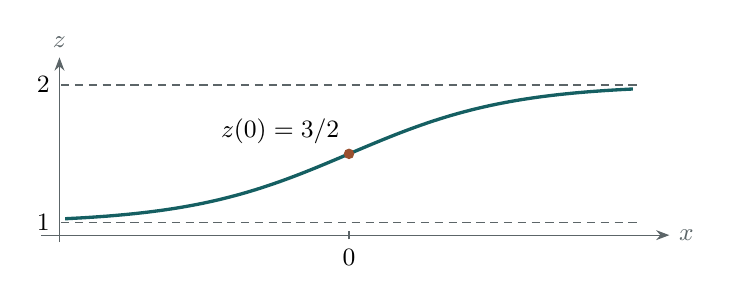
\begin{tikzpicture}[x=1.03cm,y=1.75cm,>=Stealth,font=\small]
 \draw[->,pencil] (-3.8,0.91)--(3.95,0.91) node[right] {$x$};
 \draw[->,pencil] (-3.57,.86)--(-3.57,2.2) node[above] {$z$};
 \draw[densely dashed,pencil] (-3.55,1)--(3.55,1);
 \draw[densely dashed,pencil] (-3.55,2)--(3.55,2);
 \node[left] at (-3.57,1) {$1$}; \node[left] at (-3.57,2) {$2$};
 \draw[river,very thick,domain=-3.5:3.5,samples=85] plot (\x,{1+exp(\x)/(1+exp(\x))});
 \fill[ochre] (0,1.5) circle (1.9pt);
 \node[above left] at (0,1.5) {$z(0)=3/2$};
 \draw[pencil] (0,.88)--(0,.94); \node[below] at (0,.88) {$0$};
\end{tikzpicture}
\caption{One actual solution of the slope equation. The two horizontal lines are themselves solutions. The curve between them comes from adding the two exponential modes with equal weights.}\label{fig:mixed}
\end{figure}

There are enough weights \(A,B\) to fit any initial height and slope. At zero these measurements are \(A+B\) and \(A+2B\). They determine \(A,B\) uniquely. The usual uniqueness theorem for a linear initial-value problem therefore gives the full solution \(Ae^x+Be^{2x}\)~\cite{CodLev1955}. When the quadratic has a double root \(r\), the second mode is \(xe^{rx}\). Its fractional rate is \(r+1/x\) off zero. Simply listing distinct fixed points would miss it.

\subsection{How a spring turns a growth rate into a rotation}
Give a spring a displacement \(y\). Its acceleration points back towards the middle and is proportional to that displacement. In suitable units the equation is \(y''+\omega^2 y=0\), where \(\omega>0\) sets the speed of the oscillation. The same recipe gives \(z'=-z^2-\omega^2\). A fixed point must obey \(z^2=-\omega^2\). This time both answers are imaginary, \(z=\pm\ii\omega\).

How can a growth rate be imaginary? Draw a complex number as an arrow from the origin. Multiplying by \(\ii\) turns it through a right angle. If \(y'=\ii\omega y\), the velocity is always perpendicular to the arrow from the origin. Its tip traces a circle. In symbols, \(e^{\ii\omega x}=\cos(\omega x)+\ii\sin(\omega x)\). Project that circle onto a single axis and you see a spring going back and forth. A real part of \(z\) changes the length. An imaginary part changes the angle.

More generally, write a nonvanishing wave locally as \(y=R e^{\ii\theta}\), where \(R>0\) is its length and \(\theta\) its angle. The product rule gives \(y'/y=R'/R+\ii\theta'\). We will use both readings at once when we reach Bessel.

\subsection{Euler's equation on a different clock}
Return to \(x^2\), the fourth row of the table. Its fractional rate \(2/x\) varies. But sample the curve at \(x=1,2,4,8\). Its height goes \(1,4,16,64\). Each doubling does \emph{exactly} the same thing. On the scale \(s=\log x\), consecutive doublings are the same distance apart, because \(\log(2x)-\log x=\log 2\). On that scale \(x^2=e^{2s}\) has constant fractional rate two.

The Euler equation in this paper is
\[
 (1+u)^2F''+(1+u)F'-2\ell^2 F=0.
\]
Take \(t=1+u>0\) and \(s=\log t\). The symbol \(\ell\) is a fixed number. It will acquire a physical meaning on the cone. Since \(\dif/\dif s=t\,\dif/\dif t\), the fractional rate measured with our new clock is \(W=F_s/F=tF_t/F\). Direct differentiation gives \(F_{ss}=t^2F_{tt}+tF_t\). The entire Euler equation has become \(F_{ss}-2\ell^2 F=0\), hence
\[
 \frac{\dif W}{\dif s}=2\ell^2-W^2,\qquad W^*=\pm\ell\sqrt2 .
\]
Recover the height in \(s\) and return to \(u\). This gives \(F=e^{\pm\ell\sqrt2\,s}=(1+u)^{\pm\ell\sqrt2}\). The ansatz is the coordinate change written backwards. For \(\ell=0\) the repeated exponent gives \(1\) and \(\log(1+u)\).

An equation is called \emph{autonomous} when its rule for velocity has no explicit dependence on the clock. Here the change to \(s\) made Euler autonomous everywhere on \(t>0\). It is tempting to try the very same trick on the next equation. That is where the special functions enter.

\subsection{The extra term in Bessel's equation}
Put two equations side by side. Use \(x>0\), and let the nonnegative number \(\nu\) set the power in the Euler equation.
\[
 \underbrace{x^2y''+xy'-\nu^2y}_{\text{Euler}}=0,
 \qquad
 \underbrace{x^2y''+xy'-\nu^2y}_{\text{the very same terms}}+x^2y=0.
\]
The equation on the right is Bessel's. What could one extra term do? Close to zero its coefficient is tiny. Far away its coefficient grows without bound. Euler's clock ought to work at one end. There is good reason to wonder what happens at the other.

Reuse \(s=\log x\) and write \(W=xz\). Since \(\dif/\dif s=x\,\dif/\dif x\),
\[
 \frac{\dif W}{\dif s}=xz+x^2z'
       =\nu^2-W^2-\underbrace{e^{2s}}_{x^2}.
\]
The new term has survived the change of clock. As \(s\) goes far to the left it tends to zero, leaving the Euler rule \(W_s=\nu^2-W^2\). For \(\nu>0\) the steady values of that limiting rule are \(+\nu,-\nu\). They are the fractional rates, per unit of \(\log x\), of the familiar powers \(x^\nu,x^{-\nu}\). At order zero the exponents coincide and a logarithmic solution appears~\cite{NISTBessel}.

On the ordinary \(x\) scale the same equation reads
\begin{equation}\label{eq:besselslope}
 z'=-z^2-\frac{z}{x}-1+\frac{\nu^2}{x^2}.
\end{equation}
Far to the right, for bounded \(z\), the right-hand side approaches the oscillator's rule \(z'=-z^2-1\). We have met its two steady values too, \(+\ii,-\ii\). Near one end the natural comparison is a power. Near the other it is a rotating wave. We derived both comparisons before looking up a Bessel function.

A \emph{regime} is a range of \(x\) in which particular terms dominate. An \emph{asymptotic} description tells us what becomes accurate as we go to an endpoint. If a road is straight at the beginning and straight again at the far end, knowing both bearings still leaves a great many possible roads between them. The differential equation governs the intervening stretch. To follow an actual Bessel wave, we must also say which solution we chose. We will do that in Section~\ref{sec:complex}, where one wave admits an unusually good view of the entire road.

\subsection{Where an Airy wave turns}
Bessel changes character as two terms trade importance. Airy lets us watch a change of character take place at a single point. Its equation is \(y''=xy\). For \(x>0\) a positive displacement has positive curvature, as an increasing or decreasing exponential can. For \(x<0\) the curvature points back towards zero, as it does for a spring. The change of sign at zero is why this point is called a \emph{turning point}.

The fractional-rate rule is \(z'=x-z^2\). Hold the value of \(x\) still for an instant and ask which \(z\) would give zero velocity. For \(x>0\) the answers are \(\pm\sqrt{x}\). For \(x<0\) they are \(\pm\ii\sqrt{|x|}\). These are \emph{frozen roots}. The word \emph{frozen} matters. If \(z=-\sqrt{x}\) really solved the equation, the right-hand side would be zero while the left would be \(-1/(2\sqrt{x})\).

The classical solution called \(\mathrm{Ai}\) is selected by its decay on the positive side and a conventional normalisation. Across zero, the same real solution oscillates and crosses the horizontal axis repeatedly~\cite{NISTAiry}. What becomes of \(y'/y\) at one of those crossings? That question brings us back to something we passed over in the definition.

\section{The complex plane and the trouble with zeros}\label{sec:complex}
Take the spring again. At \(x=0\) the curve \(y=\sin x\) goes through the middle at full speed. Its height is zero, its slope is one, and the spring is doing something perfectly ordinary. Yet \(z=\cos x/\sin x\) has blown up. It is our measurement that has run out of room.

A line drawn through the origin can be described by its slope until the line goes vertical. Near vertical it is easier to say how far it goes sideways for one unit up. The same trick works for the pair \((y,y')\). Near a point where \(y=0\) and \(y'\ne0\), use the reciprocal reading
\[
 w=\frac{y}{y'},\qquad
 w'=\frac{(y')^2-yy''}{(y')^2}=1+P(x)w+Q(x)w^2 .
\]
For the spring, \(z=\cot x\) and \(w=\tan x\). Near zero the second reading passes smoothly through zero with derivative one. Where both make sense they satisfy \(zw=1\). Mathematicians call these two readings \emph{charts} and the direction specified by \((y,y')\) a \emph{projective} point. Both words refer to the business of recording a direction when its overall size is irrelevant. With continuous \(P,Q\), uniqueness also tells us that a nontrivial solution cannot have \(y=y'=0\) at an ordinary point.

Bessel gives us a separate choice. Two real solutions, traditionally called \(J_\nu,Y_\nu\), can be combined into the complex wave \(H^{(1)}_\nu=J_\nu+\ii Y_\nu\). This time we \emph{are} choosing a different solution. On the positive real axis for real order, the identity \(J_\nu Y_\nu'-J_\nu'Y_\nu=2/(\pi x)\) says that the pair never vanishes together. (If they both vanished, the left side would be zero.) The combination therefore has a well-defined \(z\) there. Far from the origin it has the advancing phase \(e^{\ii x}\), up to a constant phase offset. With the usual time factor \(e^{-\ii t}\), a point of fixed phase moves outwards as time passes. This is the \emph{outgoing Hankel wave}. A real \(J_\nu\) has its own zeros and its own trajectory~\cite{NISTBessel}.

\subsection{A Bessel wave we can follow all the way}
Take order \(\nu=1/2\). Up to an overall constant the outgoing wave is~\cite{NISTBessel}
\begin{equation}\label{eq:half}
 y(x)=\frac{e^{\ii x}}{\sqrt{x}},\qquad x>0 .
\end{equation}
There is a circle in the numerator and an envelope in the denominator. One turn of the arrow takes \(2\pi\) units of \(x\) everywhere. As the arrow turns, it gets shorter. Differentiate \(x^{-1/2}e^{\ii x}\) by the product rule and divide the result by \(y\). This time both parts are visible in one line.
\begin{equation}\label{eq:halfslope}
 z=\underbrace{-\frac{1}{2x}}_{\text{fractional change in length}}
      +\underbrace{\ii}_{\text{change in angle}} .
\end{equation}
Does it really solve Bessel's equation? The derivative of the last expression is \(z'=1/(2x^2)\). With \(\nu=1/2\), the right-hand side of~\eqref{eq:besselslope} is
\[
 -\left(\ii-\frac{1}{2x}\right)^2
 -\frac{1}{x}\left(\ii-\frac{1}{2x}\right)-1+\frac{1}{4x^2}
 =\frac{1}{2x^2}.
\]
Every cancellation holds for every positive \(x\). We can now take both endpoint limits of \emph{one and the same wave}.
\[
 \begin{array}{ll}
 \text{On Euler's clock, near zero}& W=xz=-\tfrac12+\ii x\ \longrightarrow-\tfrac12.\\[2pt]
 \text{On the spring's clock, far away}& z=-1/(2x)+\ii\ \longrightarrow\ii.
 \end{array}
\]
Here is the journey the two limiting equations made us suspect. At the left end the power law records how the wave's height changes with each doubling of radius. At the right end the envelope varies so little over a turn that the wave looks locally like a pure rotation. The rotation was there even at the left end. It is the relative importance of what we measure that changes.

\begin{figure}[htbp]
\centering
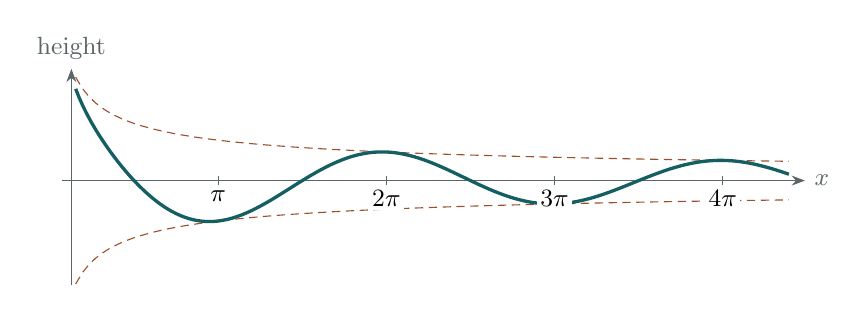
\begin{tikzpicture}[x=.68cm,y=.91cm,>=Stealth,font=\small]
 \draw[->,pencil] (.23,0)--(14.1,0) node[right] {$x$};
 \draw[->,pencil] (.4,-1.46)--(.4,1.56) node[above] {height};
 \draw[ochre,densely dashed,domain=.48:13.8,samples=110] plot (\x,{1/sqrt(\x)});
 \draw[ochre,densely dashed,domain=.48:13.8,samples=110] plot (\x,{-1/sqrt(\x)});
 \draw[river,very thick,domain=.48:13.8,samples=220] plot (\x,{cos(deg(\x))/sqrt(\x)});
 \foreach \p/\lab in {3.1416/\pi,6.2832/2\pi,9.4248/3\pi,12.5664/4\pi}{
  \draw[pencil] (\p,-.06)--(\p,.06);
  \node[below,fill=white,inner sep=1.2pt] at (\p,-.09) {$\lab$};
 }
\end{tikzpicture}
\caption{Watch the tip of the half-order Bessel wave from the side. Its horizontal projection is \(\cos(x)/\sqrt{x}\) (solid). The dashed envelope has height \(1/\sqrt{x}\) above and below the axis. The spacing of the turns stays the same as their size falls.}\label{fig:wave}
\end{figure}

Why was half-order so obliging? For most orders there is no such elementary expression for the journey. Something cancels at exactly \(1/2\). Finding that cancellation will also explain a number that keeps turning up in radial equations.

\section{The Schwarzian derivative and the Langer quarter}\label{sec:schwarz}
\subsection{First remove the changing height}
Imagine superimposing a pure oscillation on a changing envelope. If the envelope is known, we can divide it out and see the oscillation more clearly. Assume \(P\) is differentiable here. Write \(y=\mu h\), where we will choose \(\mu\). Substitution into~\eqref{eq:usual} gives
\[
 \mu h''+(2\mu'+P\mu)h'+(\mu''+P\mu'+Q\mu)h=0 .
\]
Choose \(\mu'/\mu=-P/2\). This is the recovery formula again, so we can take
\(\mu=\exp(-\frac12\int P\,\dif x)\) on our interval. The coefficient of \(h'\) vanishes. This leaves an equation in what is called \emph{normal form},
\begin{equation}\label{eq:normal}
 h''+q(x)h=0,\qquad q=Q-\frac{P'}{2}-\frac{P^2}{4}.
\end{equation}
The word \emph{potential} below just means this remaining coefficient \(q\). For Bessel take \(P=1/x,\ Q=1-\nu^2/x^2\). Then
\[
 \mu=x^{-1/2},\qquad q=1+\frac{1/4-\nu^2}{x^2}.
\]
At \(\nu=1/2\) the numerator \(1/4-\nu^2\) is zero. The rescaled wave \(h=\sqrt{x}\,y\) satisfies the spring equation \(h''+h=0\) everywhere on \(x>0\). That is where~\eqref{eq:half} came from. We can now derive it in the same direction as the classroom exponential.

\subsection{What the Schwarzian measures}
There is a second way to alter the look of a wave. Keep the same curve, but change the horizontal ruler along which its oscillations are counted. Equal steps of \(s=\log x\) correspond to larger and larger steps of \(x\). A second derivative is sensitive to that changing spacing.

Let \(s=s(x)\) be a three-times differentiable increasing ruler with \(s'>0\). Write
\(h(x)=\rho(x)H(s(x))\). Twice applying the product and chain rules gives
\[
 h''=\rho(s')^2 H_{ss}+(2\rho's'+\rho s'')H_s+\rho''H.
\]
Here the subscripts mean differentiation with respect to \(s\). We have met this choice once already. Make the middle coefficient disappear. The choice \(\rho=(s')^{-1/2}\) works, since \(\rho'/\rho=-s''/(2s')\). Differentiate that last equality once and add its square to get
\[
 \frac{\rho''}{\rho}=-\frac12\left[\frac{s'''}{s'}-\frac32
             \left(\frac{s''}{s'}\right)^2\right].
\]
The expression in brackets has a name, the \emph{Schwarzian derivative} \(\{s,x\}\). All three derivatives act on the new ruler. If \(s=2x+1\), the last two are zero, and the Schwarzian vanishes. A uniform change of scale costs nothing extra. With a nonuniform ruler, the bracket reappears in the potential of the new equation~\cite{NISTChange}.
\begin{equation}\label{eq:pull}
 H_{ss}+\widetilde q(s)H=0,\qquad
 \widetilde q(s(x))=\frac{q(x)-\frac12\{s,x\}}{(s'(x))^2}.
\end{equation}

\subsection{Where Langer's quarter comes from}
For Euler we used \(s=\log t,\ t=1+u>0\). The whole calculation takes three derivatives. With respect to \(u\), these are \(1/t,-1/t^2,2/t^3\). Thus
\[
 \tfrac12\{s,u\}
  =\tfrac12\left(\frac{2}{t^2}-\frac{3}{2t^2}\right)
  =\frac{1}{4t^2}.
\]
This is the quarter-term associated with Langer's logarithmic radial transformation~\cite{Langer1937}. To see it do some work, apply~\eqref{eq:normal} to our Euler equation. Its potential is \(q=(1/4-2\ell^2)/t^2\). In~\eqref{eq:pull} the two quarters cancel, and division by \((s')^2=1/t^2\) leaves \(\widetilde q=-2\ell^2\). We are back at the constant-coefficient equation we obtained directly. The extra quarter is the exact cost of changing the ruler while keeping a second-order equation in normal form.

\section{When can a single clock do the job?}\label{sec:autonomy}
There is now a way to test a suggested clock before solving the transformed equation. We want \(\widetilde q\) to be a constant, say \(c\). Multiply~\eqref{eq:pull} by \((s')^2\) and rearrange. The proposed clock works exactly when
\begin{equation}\label{eq:test}
 q(x)=c\,(s'(x))^2+\tfrac12\{s,x\}.
\end{equation}
If the equality holds throughout the interval, our new equation is \(H_{ss}+cH=0\) throughout that interval. It is the spring, the pair of exponentials, or, when \(c=0\), the straight line.

This suggests the working hierarchy of the original question. At \emph{level zero} the usual clock already gives a constant coefficient after the envelope is removed. At \emph{level one} a clock read from the coefficients, such as \(\log t\) for Euler, passes the test over the whole interval of interest. At \emph{level two} the simple clocks tried so far explain different ends. Order-two Bessel on \(x>0\) is a useful example. On the \(x\) clock its potential is \(1-15/(4x^2)\). On the logarithmic clock it is \(e^{2s}-4\). Each settles to a constant at one end. Neither is constant throughout.

These levels record a calculation and a choice of clocks. Change the order to \(1/2\) and Bessel drops straight to level zero. There is a further reason to specify the allowable clocks. On a real interval where two independent real solutions \(h_1,h_2\) of the normal equation are known and \(h_2\ne0\), take \(s=h_1/h_2\). Every solution then has the form \(h=h_2(As+B)\). Relative to that envelope and coordinate the shape has become a line, but constructing the ruler already required solving the problem. What I want is a ruler we can read from the equation we started with.

\section{The unification table}\label{sec:table}
Return to the last column of the opening table. This time start from equations whose solutions we may never have seen. Every row supplies \(P,Q\) for the \emph{same} rule \(z'=-z^2-Pz-Q\). Choose a row, choose the starting height and slope or the appropriate boundary data, and follow the resulting curve. In the Euler row \(t=1+u>0\). The other variable is \(x\), restricted wherever a denominator occurs.
\begin{center}\small
\begin{tabularx}{\linewidth}{@{}l l l Y@{}}
\toprule
Equation & \(P\) & \(Q\) & What to watch\\
\midrule
Constant & \(p\) & \(q_0\) & Two fixed rates give the distinct exponential modes.\\
Oscillator & \(0\) & \(\omega^2\) & An imaginary rate rotates the arrow.\\
Shifted Euler & \(1/t\) & \(-2\ell^2/t^2\) & Each doubling gives the same change of scale.\\
Bessel & \(1/x\) & \(1-\nu^2/x^2\) & A power near the origin and outgoing rotation far away.\\
Airy & \(0\) & \(-x\) & The curvature reverses its relation to height at zero.\\
Hermite & \(-2x\) & \(2n\) & The polynomial and its Gaussian-weighted wave have different rates.\\
Legendre & \(-2x/(1-x^2)\) & \(\ell(\ell+1)/(1-x^2)\) & A regular curve can have a pole in its slope chart.\\
\bottomrule
\end{tabularx}
\end{center}

Look at the last two rows. The physicists' Hermite polynomial \(H_n\) has degree \(n\). Far from the origin its leading power gives \(H_n'/H_n\) a leading term \(n/x\) when \(n>0\). Multiply it by the Gaussian \(e^{-x^2/2}\) to obtain the familiar oscillator wavefunction. Its logarithmic derivative becomes \(-x+H_n'/H_n\) by the product rule. The distinction matters if we say how the wave behaves at infinity. For Legendre take \(\ell=1\). The polynomial \(y=x\) solves the equation. Its \(z=1/x\) has a pole at zero, even though both coefficients are regular there. Conversely, the coefficients in the table are singular at \(x=\pm1\) while this particular polynomial passes straight through both~\cite{NISTPoly}.

Where does the table end? Given \(Ay''+By'+Cy=0\), enter \(P=B/A,\ Q=C/A\) wherever \(A\ne0\). For Gauss's hypergeometric equation the triple \((A,B,C)\) is \((x(1-x),\,c-(a+b+1)x,\,-ab)\). For Kummer's it is \((x,\,b-x,\,-a)\)~\cite{NISTHyper}. The same two divisions work in both cases, and both are checked in the Lean companion. This is the precise reach of the unification. On a zero-free interval every scalar homogeneous linear second-order equation has this representation, and Section~3 tells us how to return to its solutions. What singles out each family is now visible in its coefficients. What singles out a named member still lives in its boundary data.

\section{Following a moving root with WKB}
Airy's frozen roots did not solve its equation. That failed test contained a clue. On \(x>0\) we tried \(z=-\sqrt{x}\). Its derivative has magnitude \(1/(2\sqrt{x})\), while the terms \(x\) and \(z^2\) being balanced each have size \(x\). As \(x\) grows, the neglected motion is small in comparison. Could we keep just enough of it to find out how the envelope changes?

Write a normal-form equation as \(h''=p(x)^2h\) on an interval with \(p>0\). Its slope obeys \(z'=p^2-z^2\). Try following one root with a small adjustment, \(z=\sigma p+\delta\), where \(\sigma=1\) or \(-1\). Substitution gives the exact equation
\[
 \sigma p'+\delta'=-2\sigma p\,\delta-\delta^2.
\]
If \(p\) changes slowly over the local length \(1/p\), keep the first correction. Balancing \(\sigma p'\) against \(-2\sigma p\,\delta\) gives \(\delta\approx-p'/(2p)\). The recovery integral now gives
\[
 h(x)\ \approx\ \frac{C}{\sqrt{p(x)}}\exp\!\left(\sigma\int^x p(t)\,\dif t\right).
\]
This is the first WKB approximation, named for Wentzel, Kramers and Brillouin. On an oscillatory interval \(h''+p^2h=0\), the corresponding exponential carries \(\sigma\ii\int p\). The factor \(1/\sqrt p\) is what we gain by letting the root move. One can test the approximation by differentiating it in the original equation. For \(h=Ae^{\sigma\int p}\) with \(A=p^{-1/2}\), the residual \(h''-p^2h\) divided by \(h\) is exactly \(A''/A\). In particular we need that remainder small relative to \(p^2\) for this local balance to be accurate. Near a turning point \(p=0\) the formula itself tells us where to stop using it~\cite{BenOrszag1978,Olver1974}.

So far the equations have arrived already written on the page. Bessel's two regimes are especially striking once we see where its two competing terms come from.

\section{How a second variable brings Bessel into the room}\label{sec:pde}
Pick a point on a circular drumskin. Radius tells us how far it is from the centre. Angle tells us where it lies around the circle. A \emph{partial differential equation} tracks changes in both measurements. A partial derivative with respect to radius means moving outwards while holding angle fixed.

Consider a wave pattern \(\psi(r,\theta)\) on the plane satisfying the Helmholtz equation \(\Delta\psi+k^2\psi=0\). The number \(k\) sets a spatial frequency. In polar coordinates the Laplacian \(\Delta\), which measures how a function bends in space, has the form
\[
 \Delta\psi=\frac{\partial^2\psi}{\partial r^2}
  +\frac{1}{r}\frac{\partial\psi}{\partial r}
  +\frac{1}{r^2}\frac{\partial^2\psi}{\partial\theta^2}.
\]
Choose an angular pattern \(e^{\ii n\theta}\) and give it a radial amplitude \(R(r)\). This is \emph{separation of variables}. Going once round the circle must bring us back to the same value, so \(n\) is an integer. Each angular derivative contributes \(\ii n\). Cancelling the common angular factor leaves
\[
 R''+\frac1r R'+\left(k^2-\frac{n^2}{r^2}\right)R=0.
\]
There they are. The \(n^2/r^2\) term remembers how many turns the phase made on a circle of radius \(r\). The \(k^2\) term remembers the wavelength. For \(k\ne0\), rescale to \(x=|k|r\) to obtain the Bessel equation we have been following. Set \(k=0\), and Euler's equation is left. This distinction will decide what happens in the last example.

\section{Following the wave around a cone}\label{sec:coupled}
\subsection{Two people looking at the same surface}
Draw a line from near the tip of a cone towards its rim. A second observer draws a line that winds round the cone on the way out. Both can label a point by its distance outwards and an angle. What they call “keeping the angle fixed” differs. How much of the wave that the second observer sees comes from the winding of the line?

Let \(t=1+u>0\), and let \(v\) be an angle with period \(2\pi\). A \emph{metric} is the rule that turns small coordinate changes into a squared distance. In the winding coordinates take
\begin{equation}\label{eq:metric}
 \dif L^2=2\,\dif u^2+t^2(\dif v+2\pi m\,\dif u)^2,\qquad m\in\mathbb Z_{>0}.
\end{equation}
You can already see the twist. Even with \(\dif v=0\), a step in \(u\) contributes \(2\pi m\,\dif u\) to the angular bracket. Set \(\theta=v+2\pi m u\). The same ruler now reads \(\dif L^2=2\,\dif u^2+t^2\dif\theta^2\). With distance coordinate \(\sqrt2\,t\), the circumference at radius \(\sqrt2\,t\) is \(2\pi t\). That is a cone.

\subsection{Read the wave in the unwound coordinates}
A circle here has circumference proportional to \(t\). For this metric the radial part of the Laplacian is \((2t)^{-1}\partial_u(t\,\partial_u)\), and the angular part is \(t^{-2}\partial_\theta^2\). Think of the factor \(t\) as the growing circumference across which radial change is spread. Put \(\psi=F(u)e^{\ii\ell\theta}\) into \(\Delta\psi+k^2\psi=0\). The integer \(\ell\) counts the angular turns. After multiplying by two the radial equation is
\begin{equation}\label{eq:cone}
 F''+\frac{1}{t}F'+\left(2k^2-\frac{2\ell^2}{t^2}\right)F=0.
\end{equation}
First take the \emph{harmonic} case \(k=0\). We have seen this exact equation. On \(s=\log t\) it becomes \(F_{ss}=2\ell^2F\). For \(\ell\ne0\) its two modes are \(t^r\) with \(r=\pm\sqrt2\,\ell\). There was a reason to keep that fourth row on the first page.

\subsection{Read the very same wave on the winding line}
To see what the winding observer measures, put the two expressions for the angle back into the wave.
\[
 F(u)e^{\ii\ell\theta}
   =\underbrace{e^{2\pi\ii\ell m u}F(u)}_{f(u)}\,e^{\ii\ell v}.
\]
Write \(\kappa=2\pi\ii\ell m\). Wherever the wave is nonzero,
\(f'/f=\kappa+F'/F\). In the harmonic case this makes the two answers
\begin{equation}\label{eq:coneans}
 z=\kappa+\frac{r}{t},\qquad
 f(u)=e^{\kappa u}(1+u)^r,\qquad r=\pm\sqrt2\,\ell .
\end{equation}
A power law times a plane wave, globally on \(u>-1\). The power is what the unwound observer measures. Each unit of \(u\) makes the winding observer turn through \(2\pi m\) extra radians, crossing \(\ell\) angular cycles per full turn. That is the constant phase rate \(2\pi\ell m\) in the imaginary part of \(z\). When \(\ell=0\), there is no angular winding in the wave and the independent harmonic modes are \(1,\log t\).

There is a trap here that caught me in the original calculation. For \(k=0\) the equation for \(f\) has coefficients
\[
 P_f=t^{-1}-2\kappa,\qquad Q_f=\kappa^2-\kappa/t-2\ell^2/t^2 .
\]
Substitute \(z=\kappa+r/t\) into the \emph{frozen quadratic}. The result is \((r^2+r-2\ell^2)/t^2\). If \(\ell=m=1\), that quadratic offers \(r=1\). But the slope \(\kappa+1/t\) has derivative \(-1/t^2\). At \(u=0\) the right-hand side of the flow is zero while the left is \(-1\). The wave fails the very first step of its journey. Put the derivative back in before solving, and the residual becomes \((r^2-2\ell^2)/t^2\), giving exactly~\eqref{eq:coneans}. The frozen roots do get one feature right on \(\ell=m\). Their imaginary part is the constant \(2\pi m^2\). The power needs the derivative.

\subsection{Which part of the answer belongs to the coordinates?}
Keep \(k\) fixed when comparing the two observers. Multiplying \(F\) by \(e^{\kappa u}\) changes coefficients \(P,Q\) to \(P-2\kappa,\ Q-\kappa P+\kappa^2\). Indeed, direct differentiation gives
\[
 f''+(P-2\kappa)f'+(Q-\kappa P+\kappa^2)f
   =e^{\kappa u}(F''+PF'+QF).
\]
So at \(k=0\) both observers find Euler's powers. At \(k\ne0\) both retain the term \(2k^2\). Put \(x=\sqrt2\,|k|t\) in~\eqref{eq:cone} and the result is Bessel's equation of order \(\sqrt2\,|\ell|\). The observer on the winding line sees this same radial solution multiplied by the phase above. The winding explains the extra rotation exactly. The competition between wavelength and angular scale survives the change of coordinates. That distinction would have been easy to miss by looking only at the names of the functions.

\section{Where this doesn't help}
Suppose I hand you Bessel's equation and ask for the displacement of a particular drum at its rim. The slope equation alone cannot tell you which wave was excited, its size, or which condition the rim imposes. The same missing height that made \(e^x\) and \(3e^x\) indistinguishable on page one still has to come from somewhere. Boundary conditions can also couple the behaviour at opposite ends of an interval.

A second limitation is more subtle. A fixed point gives an exponential immediately, and a known Riccati trajectory gives a solution by one integral. Finding that trajectory for a new choice of coefficients can be as hard as finding the original special function. For the real Airy solution there are infinitely many zero crossings on the negative axis. Switching charts lets us continue through any ordinary crossing. It does not tell us in advance where the next crossing occurs. Those locations, the orthogonality of families and their behaviour on continuing the independent variable into the complex plane are distinct questions.

\section{Putting it to the test}\label{sec:numerical}
\subsection{What the computer algebra system does}
A calculator can make the first move much as a reader would. Its three input boxes hold \(A,B,C\), the coefficients of \(Ay''+By'+Cy=0\). Enter \(1,-3,2\). It returns the independent modes \(e^{2x},e^x\). Enter \(x^2,x,x^2-4\). It recognises Bessel of order two and returns
\[
 z'=-z^2-z/x-1+4/x^2 .
\]
The first answer supplies a basis, meaning two solutions whose linear combinations fill the solution space. The second supplies an exact reduction on a regular interval with \(y\ne0\). There is no boundary condition in those three input boxes to choose an incoming or outgoing wave. The cone operation takes \(\ell,m\) and returns the two harmonic modes, including the repeated case \(\ell=0\). To run the examples, see the \href{\caslink}{calculator instructions and supported inputs}.

\subsection{A numerical view beyond half-order}
Choose the outgoing order-two wave \(H^{(1)}_2\). Its elementary formula is no longer available to us. We can still measure the two parts of \(z=H'/H\). The real part is the fractional rate of change in length. An imaginary part approaching one means one radian of phase per unit of \(x\).
\begin{center}\small
\begin{tabular}{@{}r r r r@{}}
\toprule
\(x\)&\(\operatorname{Re}z\)&\(\operatorname{Im}z\)& Absolute residual\\
\midrule
1  & \(-1.51055\)&0.23252&\(2.01\times10^{-10}\)\\
2  & \(-0.46692\)&0.62946&\(2.28\times10^{-11}\)\\
5  & \(-0.11524\)&0.92704&\(6.75\times10^{-12}\)\\
20 & \(-0.02523\)&0.99532&\(6.01\times10^{-12}\)\\
\bottomrule
\end{tabular}
\end{center}
To reproduce the last column, evaluate \(z=\texttt{h1vp}(2,x)/\texttt{hankel1}(2,x)\) with SciPy. Estimate \(z'\) by \((z(x+h)-z(x-h))/(2h)\) at \(h=10^{-5}\). Add \(z^2+z/x+1-4/x^2\) and take the absolute value, using the unrounded values throughout. A \emph{residual} is what is left when a proposed solution goes back into the equation. These are four pointwise checks. The general large-\(x\) asymptotic for outgoing real-order Hankel waves follows from the classical expansions~\cite{NISTBessel}.

\subsection{What Lean checks}
Lean is a proof assistant. It checks a mathematical statement by following justified steps from its hypotheses. In the \href{\leanlink}{companion proof}, \(x\) is real and the solutions may be complex. Here are five places to start if you want to line up what you read with what the machine checked.
\begin{center}\small
\begin{tabularx}{\linewidth}{@{}lY@{}}
\toprule
Theorem in the Lean file & Question it answers\\
\midrule
\texttt{same\_logD\_iff\_rescaling} & Can two nonvanishing curves have the same fractional rate throughout an interval and differ by anything other than scale?\\
\texttt{half\_wave\_solves\_bessel} & Does our turning, shrinking wave satisfy the original second-order Bessel equation at every positive radius?\\
\texttt{half\_wave\_connects} & Does that very wave have both endpoint limits in Section~\ref{sec:complex}?\\
\texttt{schwarzian\_pullback}, \texttt{log\_langer} & What term enters on changing the ruler, and what does it equal for the logarithm?\\
\texttt{phase\_gauge\_residual} & What happens to the whole radial equation when the winding phase is put back in?\\
\bottomrule
\end{tabularx}
\end{center}
The file also checks the interval recovery, the reciprocal chart, the named family equations and the test for the cone exponents. All forty public theorems compile with Lean 4.26.0 and the matching mathlib release. The half-order endpoint proof is exact. The numerical values above are a separate experiment on a different order.

\section{Interpretation boundary}
Three kinds of statement have met on these pages. First are identities, such as~\eqref{eq:riccati} and~\eqref{eq:pull}, which can be run in either direction under their stated hypotheses. Second are statements about a \emph{particular} solution. For half-order we proved its connection from a single formula. For general outgoing Hankel waves or the decaying Airy function, their endpoint behaviour uses the classical results cited alongside them. Choosing which solution travels the road is part of the mathematics.

The third kind is the picture one takes away. I find it useful to ask what the two ends of a special function would call a steady rate, and whether they would measure it with the same clock. That question organised the examples here. The table encompasses many more equations than our endpoint calculations. Extending the geometric picture to a new family still requires finding the regimes, choosing a solution and showing how it travels between them.

\section{Conclusion}
What I wanted to know on the first page was who had put the exponential on the board. In the classroom example it came from a rate that could stand still. On Euler's logarithmic clock the same calculation produced a power law. Once one more term entered Euler's equation, the two ends of the problem began answering in different languages. One counted doublings. The other counted turns.

My favourite moment in this calculation is that we can hold one wave in our hands and watch it do both. Double a small radius and its length changes by a factor of \(1/\sqrt2\). Walk one full turn far from the origin and its length barely changes at all. The whole way out its fractional rate is \(-1/(2x)+\ii\). And on the cone we can ask one question more. How much of the turning belongs to the wave, and how much to the line along which we walked? Undo the twist in the ruler, and we can account for every radian.

I still do not like being asked to guess an exponential. I am quite happy to find one.

\smallskip
\noindent\textit{Companion paper.} \href{https://github.com/nickyazdani9-ux/mathematical-physics/tree/main/mathematics/contraction_integral}{\emph{The Contraction Integral}} approaches integration with a similar question about what the usual calculation lets us see.

\begin{thebibliography}{99}
\bibitem{BenOrszag1978} C.~M.~Bender and S.~A.~Orszag, \emph{Advanced Mathematical Methods for Scientists and Engineers}, McGraw-Hill, 1978.
\bibitem{CodLev1955} E.~A.~Coddington and N.~Levinson, \emph{Theory of Ordinary Differential Equations}, McGraw-Hill, 1955.
\bibitem{Ince1956} E.~L.~Ince, \emph{Ordinary Differential Equations}, Dover, 1956.
\bibitem{Langer1937} R.~E.~Langer, \href{https://doi.org/10.1103/PhysRev.51.669}{On the connection formulas and the solutions of the wave equation}, \emph{Physical Review} \textbf{51} (1937), 669--676.
\bibitem{NISTChange} NIST Digital Library of Mathematical Functions, \href{https://dlmf.nist.gov/1.13}{\S1.13, differential equations and changes of variables}.
\bibitem{NISTAiry} NIST Digital Library of Mathematical Functions, \href{https://dlmf.nist.gov/9.7}{\S9.7, Airy asymptotic expansions} and \href{https://dlmf.nist.gov/9.9}{\S9.9, zeros}.
\bibitem{NISTBessel} NIST Digital Library of Mathematical Functions, \href{https://dlmf.nist.gov/10.5}{\S10.5, Wronskians}, \href{https://dlmf.nist.gov/10.7}{\S10.7, limiting forms}, \href{https://dlmf.nist.gov/10.16}{\S10.16, half-order formulas} and \href{https://dlmf.nist.gov/10.17}{\S10.17, large-argument expansions}.
\bibitem{NISTPoly} NIST Digital Library of Mathematical Functions, \href{https://dlmf.nist.gov/18.8}{\S18.8, differential equations for the classical orthogonal polynomials}.
\bibitem{NISTHyper} NIST Digital Library of Mathematical Functions, \href{https://dlmf.nist.gov/15.10}{\S15.10, Gauss's equation} and \href{https://dlmf.nist.gov/13.2}{\S13.2, Kummer's equation}.
\bibitem{Olver1974} F.~W.~J.~Olver, \emph{Asymptotics and Special Functions}, Academic Press, 1974.
\bibitem{Reid1972} W.~T.~Reid, \emph{Riccati Differential Equations}, Academic Press, 1972.
\end{thebibliography}
\end{document}
